\documentclass[11pt,a4paper,oneside]{report}
\usepackage[utf8]{inputenc}
\usepackage[english]{babel}
\usepackage{amsmath}
\usepackage{amsfonts}
\usepackage{amssymb}
\usepackage{graphicx}
\usepackage[left=2cm,right=2cm,top=2cm,bottom=2cm]{geometry}
\author{Daniel Aguiar da Silva Carvalho}
\begin{document}
\sffamily
\begin{center}
\textbf{\large{Thesis Advancement Report 2015-2016 (Second Year)}}
\end{center}

\begin{flushleft}
\textbf{Thesis title:} Trusted-SLA Guided Data Integration on Multi-cloud Environments \\
\textbf{PhD. student:} Daniel Aguiar da Silva Carvalho \\
\textbf{Supervisor:} Chirine Ghedira-Guegan \textbf{Co-supervisors:} Nadia Bennani and Genoveva Vargas-Solar 
\end{flushleft}

\begin{flushleft}
\textbf{1 Context} \\
\end{flushleft} 

%Data integration is a widely studied issue in the database domain. It consists in merging data from different databases and providing a unified view of this data to the user~\cite{Lenzerini:2002}. Commonly, data integration is referred in the literature as a problem of answering queries using views. Many authors have reported their algorithms for this purpose~\cite{Halevy:2001}. Levy \textit{et al.} proposed the \textit{bucket algorithm}~\cite{Levy:1996}.
%Duschka and Genesereth introduced the \textit{inverse-rules algorithm}~\cite{Duschka:1997}.
%Pottinger and Halevy presented the \textit{MiniCon algorithm} in~\cite{Pottinger:2001}. \cite{Pottinger:2001} extended some ideas of~\cite{Duschka:1997}, and developed an implementation more efficient than the others.
%In general, algorithms in this domain share the same performance problem while combining views to produce a rewriting. 

Current data integration implies consuming data from different data services and integrating the results while meeting users' quality requirements. %Such requirements include the data that is retrieved and integrated, but also the properties of the data, its producers and the conditions in which such data is produced and processed. 
For example, whether the user accepts to pay for data, its provenance, veracity and freshness and how much is the user ready to pay for the resources necessary for integrating her expected result. 
%Data services provide data according to specific APIs that specify method headers with input parameters describing the data to be retrieved and the type of results they can produce. 
Moreover, data provision can be done by services according to different data quality measures. Such measures describe the conditions in which a service can provide or process data. These measures can be expressed in a service level agreement (SLA). An SLA states, what the user can expect from a service or system behavior. For example, whether it implements an authentication process, if it respects data consumer's privacy and the quality of the data the service can deliver, like freshness, veracity, reputation and other non-functional conditions like the business model that controls data delivery.

Data provision and data processing services may need a considerable amount of storage, memory and computing capacity that can be provided by cloud architectures. 
%Furthermore, users could need to integrate the data provisioned by services in a homogeneous and general result. 
%The integration process can also require important computing resources that can be obtained from the cloud too. 
%Data provision and processing services can be deployed in the cloud. 
Their SLA includes the measures about the cloud services that they require to execute their requests. The cloud, itself exports a general SLA that specifies the conditions in which users can access the services (infrastructure, platform and software) deployed in it. A user willing to use the cloud services establishes a contract with the cloud provider guided by an economic model that defines the services she can access, the conditions in which they can be accessed (duplication, geographical location) and their associated cost. Different cloud providers have different possible contracts to establish with users (i.e., platinum, silver, gold, ivory users). Thus, for a given requirement, a user could decide which cloud services (from one or several cloud providers) to use for retrieving, processing and integrating data according to the type of contracts she can establish with them.

%Data integration can be seen in the cloud computing as a service composition problem. %Selecting services and producing service compositions is computationally costly. %Moreover, executing compositions can lead to retrieve and process data collections that can require an important amount of memory, storage and computing resources. 
%%Data integration solutions on the service-oriented domain deal with query rewriting problems. 
%In our previous work~\cite{Carvalho2015}, we have identified that QoS aspects has started to considered while integrating data, and the cloud has become a popular environment to perform data integration. Moreover, data integration combined with SLA is an open issue in the cloud. 
%%In our previous work~\cite{Carvalho2015}, we have identified trends and open issues regarding the use of SLA in data integration solutions on multi-cloud environments.
%%
%Barhamgi \textit{et al.} proposed a query rewriting approach which processes queries on data provider services~\cite{Barhamgi2010}. %The query and data services are modeled as RDF views. A rewriting answer is a service composition in which the set of data service graphs fully satisfy the query graph.  
%%
%Benouaret \textit{et al.} introduced a service composition framework to answer preference queries~\cite{Benouaret2011}. In that approach, two algorithms based on~\cite{Barhamgi2010} are presented to rank the best rewritings based on previously computed scores.
%%
%Ba \textit{et al.} presented an algorithm based on \textit{MiniCon} that produces and order rewritings according to user preferences~\cite{ba2014}. %The user preference concept is a score used to rank the order in which services are selected.
%%
%As in the database domain, these approaches requires an important amount of resources to process the rewriting and integration. 
%%
%%It is important to review the existing data integration studies to be adapted to the cloud model. 

%In consequence, data consumption is determined by quality constraints specified by the user (data consumer) and different contracts (i.e., SLA's) of the clouds providing the required services. User's constraints define the storage and computing capacity of the device that consumes the data, the data transmission bandwidth and cost, whether the data consumption is critical (time constraints) and energy consumption. The SLA of the cloud determines the type of quality a user can expect from its services, according to the contract (subscription) signed between her and the cloud provider. The user profile, her quality requirements and her execution context determine the conditions in which she is expecting to consume data by using such cloud services.

Thus, the \textbf{first challenge} is to compute what we call an integrated SLA that matches the user's integration preferences (including quality constraints and data requirements) with the SLA's provided by cloud services, given a specific user cloud subscription. 
%The user may have general preferences depending on the context she wants to integrate her data such as economic cost, bandwidth limit, free services, and storage and processing limits. 
%The SLA's associated to the cloud services can be of different types: user - data service, data service - cloud provider, data provision service - data processing service, and cloud provider - cloud provider. 
In this context, matching the user' integration preferences with services can lead to an exhaustive search in the chain of SLAs and to deal with SLA incompatibilities.
Furthermore, the matching deals also with heterogeneous SLA specifications (different schemata, different measures semantics and granularities).
%, in this case it is necessary to propose a strategy to solve the problem. 
%
%The problem described in previous paragraph suggests to take into consideration the following issues:
%(i) The user may have general preferences depending on the context she wants to integrate her data such as economic cost, bandwidth limit, free services, and storage and processing limits; 
%(ii) The SLA is a contract between a service provider and a service consumer. Different entities could take place as a provider or as a consumer building, in this sense, a hierarchy of SLA such as contracts between user and the data service, data service and cloud provider, data service and data service, and cloud provider and cloud provider. In this context, matching the user integration preferences with the services that can contribute to produce a result for her can lead to search and identify in the chain of SLAs the one which contains the desired information to be matched with the user preferences, and probably it is possible to find an incompatibility between the preferences and a SLA in the chain; 
%(iii) In order to fulfill requirements and satisfy user expectations, it is possible to have a collaboration between different clouds. This collaboration implies the agreement through SLAs between services deployed in different cloud providers. In such way, matching user preferences can deal with a heterogeneity of SLA. This mean they probably do not have the same structural schema, and also the same semantic to SLA measures.  
%
%Furthermore, in order to fulfill requirements and satisfy user expectations, it is possible to have a collaboration between different clouds. This collaboration implies the agreement through SLAs between services deployed in different cloud providers. In consequence, matching user preferences with SLA's can lead to deal with heterogeneous SLA specifications (different schemata, different measures semantics and granularities). Computing an integrated SLA can imply dealing with heterogeneous SLA specifications and SLA-preferences incompatibilities.

The \textbf{second challenge} is to guide data integration taking into consideration the integrated SLA. Here, the data integration process includes (i) looking up services that can be used as data providers, and for services required to process retrieved data and build an integrated result; (ii) performing data retrieval, processing and integration and (iii) deliver results to the user considering her preferences (quality requirements, context and resources consumption). The integrated SLA guides services selection and filtering; it can help to control the amounts of data to retrieve and process according to consumption rights depending on the user subscription to the participating cloud providers and how to deliver data considering the user's context.

%The cloud computing paradigm provides computing resources (as services) in an on-demand and scalable manner to cloud consumers. This on-demand provision and the pricing model imposed by the cloud changes the way data integration solutions should be tackled. Instead of designing processes and algorithms taking into account the limits on resources availability, the cloud sets focus on the economic cost allowing resource consumption and producing results while delivering data under subscription oriented cost models.

%When a service is billed to a consumer, the provider and customer agree on price, quality guarantees and penalties associated to its violation in service level agreement (SLA) contracts. 
%Several researches have reported their studies on SLA in different domains~\cite{AlhamadDC11}. In the cloud context, Rak \textit{et al.} proposed an approach to specify security requirement and to associate them to cloud services~\cite{rak2013}. Mavrogeorgi \textit{et al.} introduced a SLA management framework that allows the creation and enforcement of customized SLAs~\cite{Mavrogeorgi2013}. Leitner \textit{et al.} presented an approach to monitor and predict SLA violations before they impacted the provider's SLA~\cite{Leitner2010}. In general, proposals regarding SLAs in the deployment of services focus on two aspects: (\textit{i}) approaches focusing on the life cycle of the SLA mainly interested in the contract negotiation phase between the cloud and the service consumer; and (\textit{ii}) works monitoring contracts and cloud resources in order to avoid SLA violations, and consequently penalties due to its violation. In this sense, to the best of our knowledge, we have not identified any other approach that proposes the use of SLA associated to a data integration solution in a multi-cloud environment.

%With growing needs and requirements, applications use different cloud providers for externalizing different data processing and management resources. This fact adds more challenges to data integration considering (i) the large amount and diversity of data; (ii) the user quality and security requirements of the integration; and (iii) the cloud heterogeneity in expressing and enforcing the corresponding clauses. Indeed, we believe that given the volume and the complexity of query evaluation, it is important to combine and revisit well-known data integration solutions and adapt them to this context. We strongly believe that this can be done according to quality of service requirements expressed by the consumers and service level agreement contracts exported by the cloud providers that host data collections and deliver resources for executing the associated management processes.

This thesis project intends to address data integration in a multi-cloud hybrid context. The originality of our approach consists in guiding the entire data integration solution taking into account (i) user preferences statements; (ii) SLA contracts exported by different cloud providers; and (iii) several QoS measures associated to data collections properties (for instance, trust, privacy, economic cost). The objective is to propose data integration strategies adapted to the vision of the economic model of the cloud.
%
In our work we consider an example from the domain of energy management. My directors are working on two national projects in this domain. So for instance, we assume we are interested in queries like: Give a list of energy providers that can provision 1000 KW-h, in the next 10 seconds, that are close to my city, with a cost of 0,50 Euro/KW-h and that are labeled as green? The question is how can the user efficiently obtain results for her queries such that they meet her QoS requirements, they respect her subscribed contracts with the involved cloud provider(s) and such that they do not neglect services contracts? Particularly, for queries that call several services deployed on different clouds. 
%This work is part of an international collaboration with the DiMAp, Federal University of Rio Grande do Norte.
 
\begin{flushleft}
\textbf{2 Synthesis and Perspectives of the Research Activities}\\
\end{flushleft}
During the second year, we have organized our research activities as follows:

\noindent \textbf{Development of our data integration approach}. Given a query and a set of user preferences associated to it, the query execution process is divided in three phases. 
%The figure 1 illustrates our data integration approach.
%\begin{figure}[h!]
%\center
%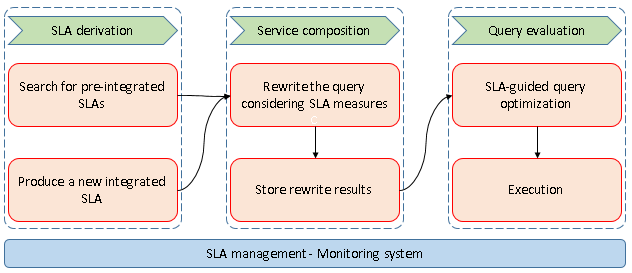
\includegraphics[scale=0.7]{../../general_approach.PNG} 
%\caption{SLA-guided data integration approach}
%\end{figure}
\underline{The first phase} is the \textsl{SLA derivation} in which a SLA for the user request is created. It consists in looking for a (stored, integrated) SLA derived for a similar request. If a similar SLA is found, the request is forwarded to the query evaluation phase. Otherwise, a new SLA to the integration (called integrated SLA) is produced. The query is expressed as a service composition with associated user preferences. In \underline{the second phase}, service composition, the query is rewritten in terms of different services considering the user preferences and the SLAs of each service involved in the composition. The rewriting result is stored for further uses. \underline{Finally}, in the query evaluation phase, the query is optimized in terms of user preferences and SLAs concerning the consumed resources and the economic cost of the query. Once optimized, the query processed in the execution engine. In addition, we are assuming a SLA management module and monitoring system responsible to verify if the SLA contracts are being respected. %Firstly, we have worked on the phases two in order to have an algorithm that will allow us to run important experiments to evaluate our approach. 
%The following activities were developed to achieve our objectives:

\noindent \textbf{Extension of the query rewriting algorithm}. In collaboration with our colleagues in Brazil (authors in~\cite{ba2014}), we have worked on an adapted version of \cite{ba2014} to our data integration solution extending their data structure to map services to the query, and adding the concepts of user preferences to the query and quality measures to the services. In addition, we have developed and formalized the \textit{Rhone} service-based query rewriting algorithm guided by service level agreements (SLA). Our work proposes two original aspects: (i) the user can express her quality preferences and associated them to his query; and (ii) service's quality aspects defined in SLAs guide the service selection and the whole rewriting process taking into consideration that services and rewritings should meet the user requirements, and the different cases of incompatibilities of SLAs, uncompleted SLA and the integration SLA. Preliminary experiments were produced to evaluate the \textsl{Rhone}.

%However, while performing the integration we have identified some design issues that made it useless to our approach: (i) their concept of user preferences are scores associated to services previous defined by the user while, for us, user preferences are quality requirements expected by the user concerning the whole integration; (ii) their algorithm accepts rewriting including calls to services that are not interest for the composition. Assuming that on the cloud each service has a price associated to its request, these composition that calls useless services produces an extra cost to the user. This adaptation process helped us to identify important issues to be applied to our own implementation such as developing an better approach to produce the combinations of services.

%a) Adapting a previous query rewriting algorithm to our approach. This work was performed in collaboration with our colleagues in Brazil. The idea was to adapt a previous work from their lab to our data integration solution. While integrating we have identified some design problems that made it useless to our approach. However, the work in group help us to identify important issues to be applied to our own implementation.

%b) Query rewriting algorithms. We have produced a state of the art about query rewriting algorithm.  The approaches are divided into two different domains: database and service-oriented architecture. In the database domain, the different works concerning query rewriting using views have been studied in the literature. In general, the approaches deal with an exponential problem depending on the size of the query and the quantity of views. In the service-oriented domain, the approaches share the same problem. Producing services composition is extremely costly depending on the size of the composition (query) and the amount of services to be combined. Some approaches have tackled this issue. They have tried to minimize the effort to produce rewritings by considering user preferences or by limiting the desired number of rewritings. These works have been used as base and reference to produce our own algorithm.

%Starting from the knowledge acquired while working on~\cite{ba2014}, we have produced a state of the art about query rewriting algorithm. The approaches can be divided into two domains: database and service-oriented architecture. In the database domain, studies (such as \cite{Duschka:1997,Levy:1996,Pottinger:2001}) have documented their approaches for answering queries using views. In general, while producing rewritings, these approaches suffer from the time exponential problem depending on the size of the query and the quantity of views. In the service-oriented domain, query rewriting can be seen as a service composition problem. Approaches (such as \cite{Barhamgi2010,Benouaret2011,Umberto}) share the same problem as on the database domain while producing services composition which is a task extremely costly depending on the size of the composition (query) and the amount of services to be combined. \cite{ba2014} have tried to minimize the effort to produce rewritings by considering user preferences (as scores) and by limiting the desired number of rewritings.

%Based on the related work, we have developed and formalized the \textit{Rhone} service-based query rewriting algorithm guided by service level agreements (SLA).
%Based on the related work, we have developed and formalized the \textit{Rhone} service-based query rewriting algorithm guided by service level agreements (SLA). The \textit{Rhone} assumes that there are a set of quality measures associated to services which we suppose they are previously extract from their SLA. These measures will guide the service selection and the entire rewriting process.  Our work address this issue and proposes the algorithm with two original aspects: (i) the user can express her quality preferences and associated them to his query; and (ii) service's quality aspects defined in SLAs guide the service selection and the whole rewriting process taking into consideration that services and rewritings should meet the user requirements, and the different cases of incompatibilities of SLAs, uncompleted SLA and the integration SLA. 
%and (ii) while trying to fulfill the user quality preferences, service’s quality aspects defined in SLAs guide the service selection and the whole rewriting process (Services and rewritings should meet the user requirements).
%Given a set of abstract services, a set of concrete services and a user query (both defined in terms of abstract services), and a set of user quality preferences, the \textit{Rhone} derives a set of service compositions that answer the query and that fulfill the quality preferences regarding the context of data service deployment. The algorithm consists in four steps: (i) \textit{Selecting concrete services}. Similar to~\cite{Levy:1996,Pottinger:2001} our algorithm selects services based on the abstract services that exists in the query, but it includes two differences: first, a concrete service cannot be select if it contains an abstract service that is not present in the query; and second, the service' quality aspects (extracted from its SLA) must be in accordance with the user quality preferences; (ii) \textit{creating mappings from concrete services to the query (called concrete service description (CSD))} inspired in~\cite{Pottinger:2001} including also the information concerning the services' SLA; (iii) \textit{combining CSDs}; and (iv) \textit{producing rewritings} until fulfilling the user requirements according to the services' SLA. Each phase of the algorithm and each concept (query, concrete services, mapping rules, for instance) were formally specified and described.

%d) Configuration of a multi-cloud environment. We have worked on the configuration of a multi-cloud environment. However, we found some problems at this point: (i) the configuration and deployment of cloud infrastructure using open source technologies is not easy and requires important technical skills while configuring the network resources; (ii) it requires a powerful machine. Due to that we have configured a simulation of cloud; and (iii) we have searched for private cloud providers, but they allow few access and power permissions to manage resources. In addition, they are quite expensive. We are still working on best way to manage this issue.

%In order to evaluate our approach and the \textit{Rhone} algorithm, we began configuring a multi-cloud environment. We have searched for open source solutions instead of privates once they are (i) quite expensive; and (ii) do not allow to extend and access directly the different level of SLAs. The OpenStack was selected as our technology. We have installed and configured the different modules necessaries to the OpenStack. However, we have some issues: (i) the configuration and deployment of cloud infrastructure require important technical skills while configuring the network resources; (ii) it requires a powerful machine. Due to these reasons we have configured a simulation of cloud run our experiments.

%The first version of the \textit{Rhone} was implemented using Java according to its formal definition. The algorithm was tested in a cloud simulation containing 35 services in its service registry. We have tested different types of query varying on the size and on the number of user preferences. Although our algorithm shares the same time performance problem as the previous approaches while combining compositions, the preliminary experiments have shown that the Rhone can enhance the quality in data integration by considering the user preferences and service’s quality aspects extracted from service level agreements. Our approach avoid selecting and using services to produce compositions that are not interest to the user once they do not fulfill his quality requirements. In addition, as result we have submitted short paper to EDBT 2016. 

%We developed an improved version of the algorithm that better manages the manner in which lists of objects are managed. We have applied this version to a new set of experiments running 100 concrete services. With the results obtained from this experiment and the final version of our formalization, we are working on a new paper that included an extensive description of the algorithm and its evaluation to be submitted to ADBIS 2016 (deadline 27th March).

%h) SLA model to data integration. The state of the art on SLA have been analyzed to serve as basis to our SLA model. The works on SLA to cloud computing can be divided in two groups: (i) approaches dealing with the SLA negotiation phase. They focus on methods to stablish good and well-defined agreements between providers and customers; and (ii) works focus on monitoring/allocating resources in order to detect and avoid SLA violations. These works helped while proposing our SLA model and schema. Note that the SLA is the main concept in our proposal. It is responsible to guide the entire approach from the beginning to the end. There are some challenges regarding SLA: (i) once we are inserted into a multi-cloud context, we are dealing with a large heterogeneity of SLAs among different clouds. It is possible to have the same concept defined in a different way depending on the cloud; (ii) there are different levels of SLA: user SLAs, service SLAs and cloud SLAs. It is necessary to have a mapping between SLA measures that can be expressed in a different manner depending on the level; and (iii) it is possible to face a diversity chain of SLA from different levels and to map and identify measures is a hard process.

Currently, we have been working on the SLA model to data integration, on the schema for user SLA, cloud SLA and integration SLA, and on a scenario description to illustrate our approach.  %The result of this work is going to be described in a VLDB PhD workshop (to be submitted until 4 April).

%With this work performed, we have been designing our SLA model to data integration. As mentioned before, proposals to SLA in cloud computing can be divided in two groups: (i) approaches dealing with the SLA negotiation phase. They focus on methods to establish good and well-defined agreements between providers and customers; and (ii) works focus on monitoring/allocating resources in order to detect and avoid SLA violations. These works helped us while proposing our SLA model and schema. The SLA is the main concept in our proposal. It is responsible to guide the entire approach from the beginning to the end while fulfilling the user requirements. At this point, some challenges arises: (i) In a multi-cloud context, we are dealing with a large heterogeneity of SLAs among different clouds in terms of semantics and structure. A SLA and its measure can be defined in a different way depending on the cloud; (ii) there are different levels of SLA: between users and services, between services and clouds, between clouds and clouds. Consequently, a user requirement defined in a user SLA is computed in terms of different measures on Service and Cloud SLAs. It is necessary to have a mechanism that maps and compute the user requirement and SLA measures; and (iii) it is possible to exists a chain of SLA, and to map and computed measures in this chain can require a hard processing. i) Paper to ADBIS and VLDB PhD consortium. Currently, we have been working on a paper that focus on the description of our SLA model, schema and data integration approach to be submitted to the VLDB PhD workshop (deadline 4 April).

%i) Paper to ADBIS and VLDB PhD consortium. Currently, with our last results, we have been working on two new papers: one concerning the algorithm to be submitted to ADBIS 2016 (deadline 27th March), and another one focusing on the SLA model, schema and data integration approach to be submitted to the VLDB PhD workshop (deadline 4 April).

\noindent
\textbf{Publications}.
D. A. S. Carvalho, P. A. Souza Neto, G. Vargas-Solar, N. Bennani, C. Ghedira, Rhone: a quality-based query rewriting algorithm for data integration, Short paper, {\em 20th East-European Conference on Advances in Databases and Information Systems}, ADBIS 2016 (to appear).

%\noindent
%Additionally, in April, I attended to the \emph{1st French Brazilian School on Smart cities and Big Data} at the University of Grenoble Alpes (http://fr-br-school.imag.fr).

%Once we have been working on the second phase of our data integration approach, we are going to carry on completing what is missing on the other phases. This concerns to (i) propose the user, service and cloud SLA schema for data integration; (ii) develop and describe our data integration architecture; and (iii) build the module that threats the SLA and extracts its measures information to be used in the \textit{Rhone} rewriting algorithm. As we mentioned before, the work concerning the SLA is the core of our approach. Here, while matching user preferences with SLA's, we are dealing with heterogeneous SLA specifications (different schemata, different measures semantics and granularities), different cases of  SLA specifications and SLA-preferences incompatibilities. In addition, an optimization of our algorithm is also necessary to be able to process a huge amount of services.

%With this work done, we are going to integrate both parts: the SLA module and the Rhone algorithm. The evaluation of the approach is essential and it can be presented to partners in energy domain to validate the feasibility of our approach. Once the modules are connected, a set of experiments in a multi-cloud environment will be performed to evaluate our solution. The results analysis will be the basis to another scientific article. In parallel, we will start writing the thesis document. The table below describes our intended calendar. In green, you can see activities that we have done (previously described in the section 2). In blue, future activities.

%The following activities are:
%\begin{enumerate}
%\item Paper submission ADBIS: this paper aims to present the description and formalization of the Rhone service-based query rewriting algorithm, and the results of the experiments produced in a cloud simulation.
%\item Paper submission VLDB PhD workshop: this paper describes our data integration approach focusing on the SLA model and schema.
%\item Building the SLA Module. The idea is to implement the module responsible (i) to use the SLA model proposed and (ii) to extract information from a diversity of SLA and produce the inputs required to our rewriting algorithm.
%\item Optimizing the Rhone algorithm. The goal is to minimize the loss in performance and show that our algorithm gain in time while avoiding to selecting and composing services that clearly violate the user preferences.
%\item Integrating modules. The aim is to integrate the SLA module and the Rhone algorithm.
%\item Producing and evaluating experiments. Once the different modules and the three phases of the approach are working integrated, experiments are going to be performed in a simulation of multi-cloud to evaluate the entire solution.
%\item Producing a scientific paper. Naturally, the results obtained from the previous experiments is going to be used in another scientific production.
%\item Writing the thesis.
%\end{enumerate}

\begin{figure}[h!]
\center
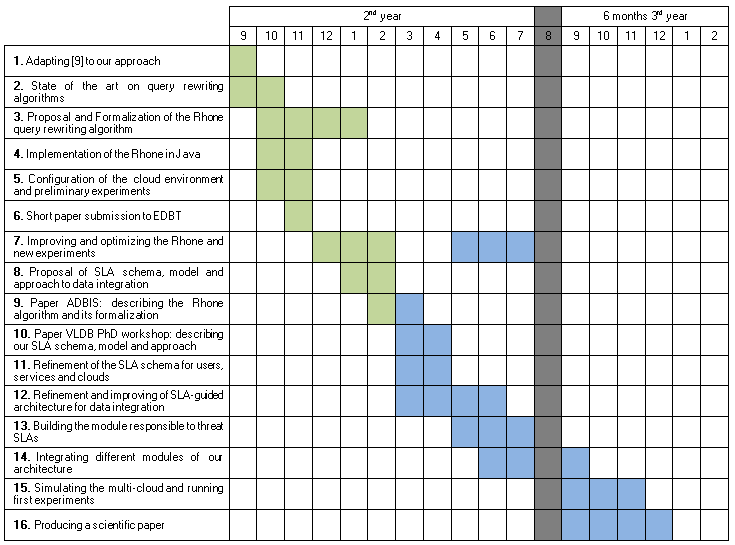
\includegraphics[scale=0.7]{calendar.png}
\end{figure}

\noindent
The figure below presents the perspectives described as activities in the following calendar. 

\bibliography{report}
\bibliographystyle{plain} 

\end{document}